\section{Stromleitung auf der Atomarer Ebene}
Strom fließt in einen Leiter, z.B ein Kupferdraht, indem sich Elektronen durch das Leitermaterial
bewegen. Elektrische Leiter bestehen aus positive geladenen Ionenrümpfe\footnote{Ionenrümpfe sind die Atome des Kristallgitters, die eines oder mehrere ihrer außen Elektronen abgegeben haben und deswegen positiv geladen sind}, die in einem Kristallgitter angeordnet sind. Um 
die Ionenrümpfe befinden sich die Elektronen welche wie in einem Gas frei um die Ionenrümpfe herum fliegen.


\begin{figure}[h]
    
    \centering
    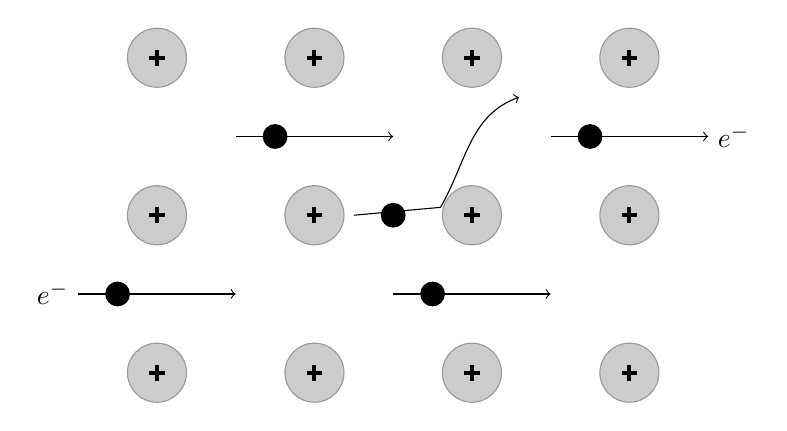
\begin{tikzpicture}
        % Zeichne die Ionenrümpfe als Kreise im Kristallgitter
        \foreach \x in {0,2,4,6} {
            \foreach \y in {0,2,4} {
                \node[circle, draw=gray!80, fill=gray!40, minimum size=7.5mm] at (\x,\y) {};
                \draw[line width=0.5mm] (\x-0.1,\y) -- (\x+0.1,\y);
                \draw[line width=0.5mm] (\x,\y-0.1) -- (\x,\y+0.1);
            }
        }
        
        % Zeichne Elektronen als kleine blaue Kreise mit Pfeilen für Bewegung
        \foreach \pos in {(-0.5,1), (1.5,3), (3.5,1), (5.5,3), (3,2)} {
            \filldraw[black] \pos circle (0.15);
        }
        \draw[black,->] (-1,1) node[left]{$e^-$} -- (1,1);
        \draw[black,->] (1,3) -- (3,3);
        \draw[black,->] (3,1) -- (5,1);
        \draw[black,->] (5,3) -- (7,3) node[right]{$e^-$};
        
        % Stöße der Elektronen mit den Ionenrümpfe
        \draw[black,->] (2.5,2) -- (3.6,2.1) to[out=60,in=200] (4.6,3.5);
        
    \end{tikzpicture}
    \caption{Elektronengas in einem Leiter}
    \label{fig:Elektronengas}
\end{figure}
Legt man eine Spannung an bewegen sich die Elektrone von minus Pol zum plus Pol 
wobei sie mit den Ionenrümpfe zusammenstoßen, wie in Abbildung \ref{fig:Elektronengas} dargestellt.
Durch diese Stöße werden die Elektronen gestreut was den Stromfluss behindert und so zu einem Wiederstand führt. Die Gitter Schwingungen 
hängen von der Temperatur ab, desdo höher die Temperatur, desdo stärker die Schwingungen und desdo mehr Stöße gibt es, was zu einem höheren
Widerstand führt. Umgekehrt ist das natürlich 
auch der Fall. \\

Bei bestimmten Metallen, wie z.B. Quecksilber oder Blei, kann man aber beobachten das der Wiederstand ab einer bestimmten 
Temperatur plötzlich ganz verschwindet. Dieses Phänomen kann durch die BCS-Theorie erklärt werden.